\chapter{Ambientes de Testes}

\section{Introdução}

O estudo em segurança cibernética tem um início lento e difícil por inúmeros motivos, dentre eles a necessidade de bases em outras áreas para uma compreensão do que é feito para explorar determinadas vulnerabilidades, além disso, existe a necessidade de amparo legal para as ações referentes aos testes de vulnerabilidades realizados. Não é possível apenas testar uma vulnerabilidade em um site qualquer, pois tais testes podem ser interpretados como uma tentativa de invasão e levar a problemas legais. E por isso ambientes de teste tem muitas utilidades dentro de cada tema explorado para estudo.

Parte das dificuldades encontradas na área de aprendizado de segurança cibernética podem ser sanadas pela utilização de um ambiente de teste. Obviamente o mesmo não tem o mesmo valor que uma aplicação real, mas pode ser muito útil para pessoas que querem testar novas ferramentas, explorar novas vulnerabilidades ou iniciar o seu estudo na área da segurança da informação. Um ambiente de teste, consegue isolar os testes para a própria máquina local e isso na segurança da informação é muito importante já que não é possível para \textit{pentesters} ou profissionais que estejam testando vulnerabilidades que eles façam estes testes em aplicações reais sem as devidas permissões. Ao mesmo tempo, nem sempre é a melhor opção realizar determinados testes na aplicação real, já que pode gerar custos desnecessários e perdas econômicas no caso do serviço ficar indisponível. Então profissionais de segurança da área defensiva da segurança da informação podem usar destes ambientes para entender melhor certas falhas e então com base nisto aperfeiçoar seus próprios sistemas sem ter que colocar em um primeiro momento seus sistemas a prova. Portanto, um ambiente \textit{Sandbox} para testes de vulnerabilidade se torna útil não apenas aos profissionais que querem se aperfeiçoar no ataque de sistemas, mas também aos que querem melhorar a segurança de alguma aplicação. 

%quais ambientes existentes

Hoje existem vários ambientes de segurança que podem ser utilizados para a realização de testes de vulnerabilidade desenvolvidos com diversas tecnologias, os mais comuns são como aplicações web ou imagens para máquinas virtuais. Este teste descreverá trabalhos desenvolvidos como imagens de sistemas com aplicações executando internamente, uma vez que nestes ambientes existem falhas de segurança web que podem resultar em problemas mais graves como vulnerabilidades em redes e/ou em sistemas operacionais. Tanto a OWASP BWA quando a Mutillidae II são bons exemplos de imagens com falhas muito interessantes.


\section{OWASP Broken Web Applications}

O BWA (OWASP Broken Web Applications) é um projeto da OWASP para auxiliar na exploração e aprendizado de falhas de segurança, no teste de ferramentas automatizadas, na observação de ataques em aplicações web, no teste de técnicas de avaliação manual e no teste de WAFs (Web Application Firewall) \cite{url:OWASPBWA}. A Figura 1 representa a \textit{homepage} da imagem BWA.

\begin{figure}[!htb]
     \centering
     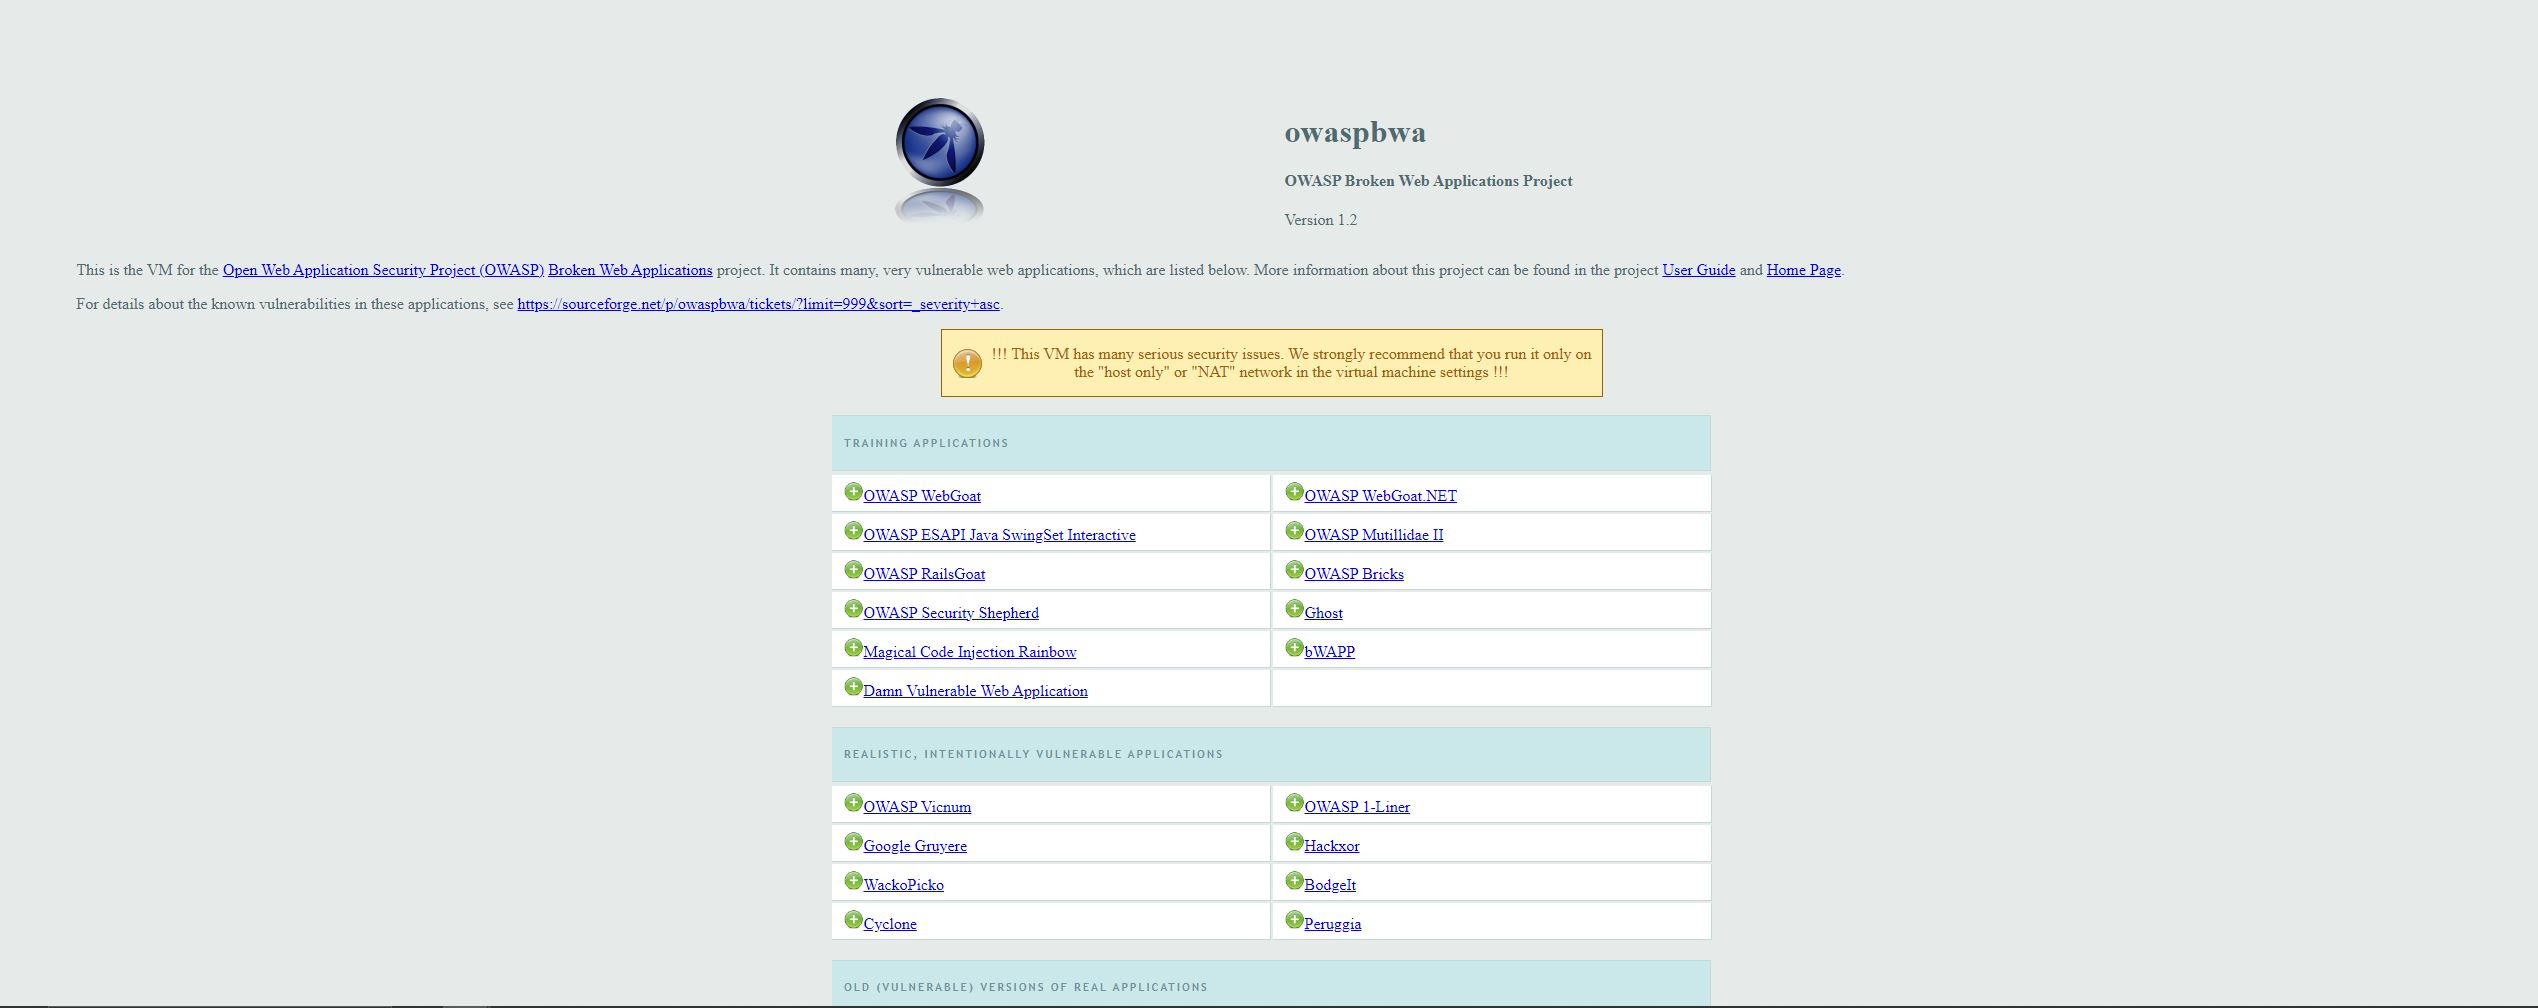
\includegraphics[width=15cm]{OWASPBWA.JPG}
     \caption{Captura de tela da OWASP BWA}
     \label{Label de referência para a imagem}
\end{figure}

\section{Mutillidae II}

A Mutillidae II é uma aplicação web open-source que oferece mais de 40 vulnerabilidades e desafios com vulnerabilidades encontradas desde a OWASP TOP Ten de 2007 até a de 2017. O ambiente conta com tutoriais e dicas para auxiliar no aprendizado e possui várias falhas simples de sempre exploradas para estimular o aprendizado da área \cite{url:owaspmuti}. Na Figura 2 é possível ver uma das páginas da Mutillidae II.

\begin{figure}[!htb]
     \centering
     \includegraphics[width=15cm]{Questão8.JPG}
     \caption{Captura de tela da Mutillidae II}
     \label{Label de referência para a imagem}
\end{figure}

%mutillidae 2